 \documentclass[5]{article}
\usepackage[utf8]{inputenc}
\usepackage{hyperref} 

\usepackage[T1]{fontenc}
\usepackage[polish]{babel}

\title{Laboratorium 9}
\author{Piotr Witek}
\date{19 maja 2021}

\usepackage{natbib}
\usepackage{graphicx}
\usepackage{geometry}
\usepackage{tabularx}
\usepackage{array}
\usepackage{amsmath}

\begin{document}

\newgeometry{tmargin=2cm, bmargin=2cm, lmargin=2.5cm, rmargin=2.5cm}

\maketitle


\section{Zadania}

\hspace{4mm} \large \textbf{Tematem zadania będzie obliczanie metodami Monte Carlo całki funkcji $x^2$ oraz $1/sqrt(x)$ w przedziale (0,1). Proszę dla obydwu funkcji:}
\newline

\subsection{Napisać funkcję liczącą całkę metodą "hit-and-miss". Czy będzie ona dobrze działać dla funkcji $1/sqrt(x)?$}

\vspace{5mm}

Funkcję liczącą całkę metodą Monte Carlo napisałem w języku Python. Jej kod to:

\begin{verbatim}
    def monteCarlo(N):
    x = np.random.uniform(low = 0, high = 1, size = [N, 1])
    y = np.random.uniform(low = 0, high = 1, size = [N, 1])

    smaller_bool = x**2 > y
    # smaller_bool = 1/math.sqrt(x) > y

    approx = np.sum(smaller_bool)/N
\end{verbatim}

\vspace{5mm}
Następnie, zarówno dla funkcji $x^{2}$ oraz $1/sqrt(x)$ wykonałem napisaną wyżej funkcję.
Okazuje się, że metoda 'hit and miss' nie działa dobrze dla drugiej funkcji. Podejrzewam, że wynika to z faktu iż funkcja ta ma granicę dążącą do nieskończoności przy 0+.
\vspace{4mm}

\subsection{Policzyć całkę przy użyciu napisanej funkcji. Jak zmienia się błąd wraz ze wzrostem liczby podprzedziałów? Narysować wykres tej zależności przy pomocy Gnuplota. Przydatne będzie skala logarytmiczna.}


Następnie wykonałem funckję całkującą dla funckji $x^2$ dla wartości podprzedziałów z tablicy poniżej:
\begin{verbatim}
    [5, 10, 50, 100, 500, 1000, 5000, 10000, 50000, 100000, 500000, 1000000]
\end{verbatim}

Wyniki programu kształtują się w sposób następujący:
\begin{verbatim}
    0.4
    0.3 
    0.42
    0.39
    0.322
    0.335
    0.3428
    0.3345
    0.3281
    0.33468
    0.33251
    0.334158
\end{verbatim}

Znając faktyczną wartość calki na przedziale (0,1) wynoszącą 1/3, zauważam, że wraz z wzrostem liczby próbek, dokładność wyników zwiększa się. Warto zwrócić jednak uwagę, że ciągłe zwiększanie liczby N - liczby popdprzedziałów, nie ma większego sensu. Generator liczb pseudolosowych ma skończonie wiele liczb w cyklu.

\vspace{4mm}
Do pliku data.txt zapisałem wyniki działań funkcji w formacie (N - liczba podprzedziałów, sigma - błąd wyrażony w procentach). Uzyskane wyniki prezentują się następująco:
\begin{verbatim}
    5 80.0
    10 20.00000000000001   
    50 8.000000000000002   
    100 11.000000000000004 
    500 0.20000000000001128
    1000 2.6000000000000134
    5000 2.2600000000000007
    10000 1.0599999999999998 
    50000 0.39999999999998925
    100000 0.08600000000001384
    500000 0.10479999999999379
    1000000 0.07789999999999742
\end{verbatim}
\vspace{4mm}

Następnie wykonałem wykres zależności N do sigma. Który prezentuje się w taki sposób:

\begin{center}
    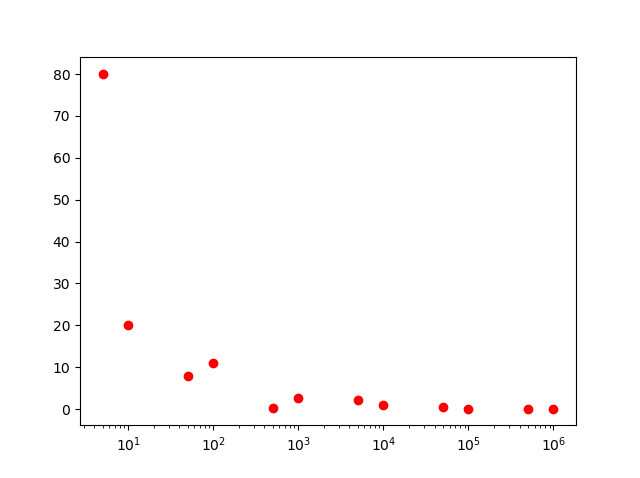
\includegraphics[scale=0.7]{Figure_1.png} \par
    \vspace{3mm}
\end{center}

Można łatwo zauważyć, że błędy całkowania wraz ze wzrostem N - liczby podprzedziałów, maleją odwrotnie proporcjonalnie do pierwiastka z liczby próbek, czyli $1/sqrt(N)$
\vspace{5mm}




\section{Bibliografia}

\begin{enumerate}
  \item \url{https://www.gnu.org/software/gsl/doc/html/montecarlo.html}
  \item \url{https://mathworld.wolfram.com/MonteCarloMethod.htmle}
  \item \url{https://www.taygeta.com/rwalks/node3.html}
\end{enumerate}

\end{document}

